最適化の方法として,複数のパラメータからモデル,実行環境に即したパラメータを選択するという手法を選択したが,
そのためには複数のパラメータでシミュレーションを行いその結果を集約するプログラムが必要となる.\\
本研究ではこのパラメータ選択を容易かつ高速に行うため以下に示すプログラムを作成した.\\
・MODファイルからパラメータとなりうる変数を自動で抽出し,それぞれの関係性を元に配列とその順序の候補を生成する.\\
・ジョブキューのシステムを持っているマシンにおいて,複数のジョブを並行して投げ結果を非同期的に集約できる.\\
・実行結果を最適化前のデフォルトの結果と比較し,実行結果に対して影響がないかを確認する.\\
・json形式で実行するファイル,各パラメータの範囲(プロセス数は1から10など)を指定することができる.\\
\subsubsection{全体構成}
はじめにシミュレータプログラムを構成する要素について示す.\\
( TODO: 章番号)にあるアルゴリズムで述べたように,探索の対象となるパラメータは,モデルに依存するパラメータ,
実行マシンに依存するパラメータそしてコンパイルに関わるパラメータの3つに大別される.\\
そのうち,モデルとコンパイルに関わるパラメータは実行形式の生成に関与し,実行マシンに関わるパラメータは
ジョブスクリプトの生成に関わる.\\
実行形式とジョブスクリプトそれぞれの生成にかかる時間は表 ( TODO: 表を作る)のようになり,スーパーコンピュータ京,研究室クラスタ
双方において実行形式の生成にかかる時間が多いことがわかる. よって\\
\begin{figure}[htb]
% h:here, t:top, b:bottom, p:page
  \begin{center}
    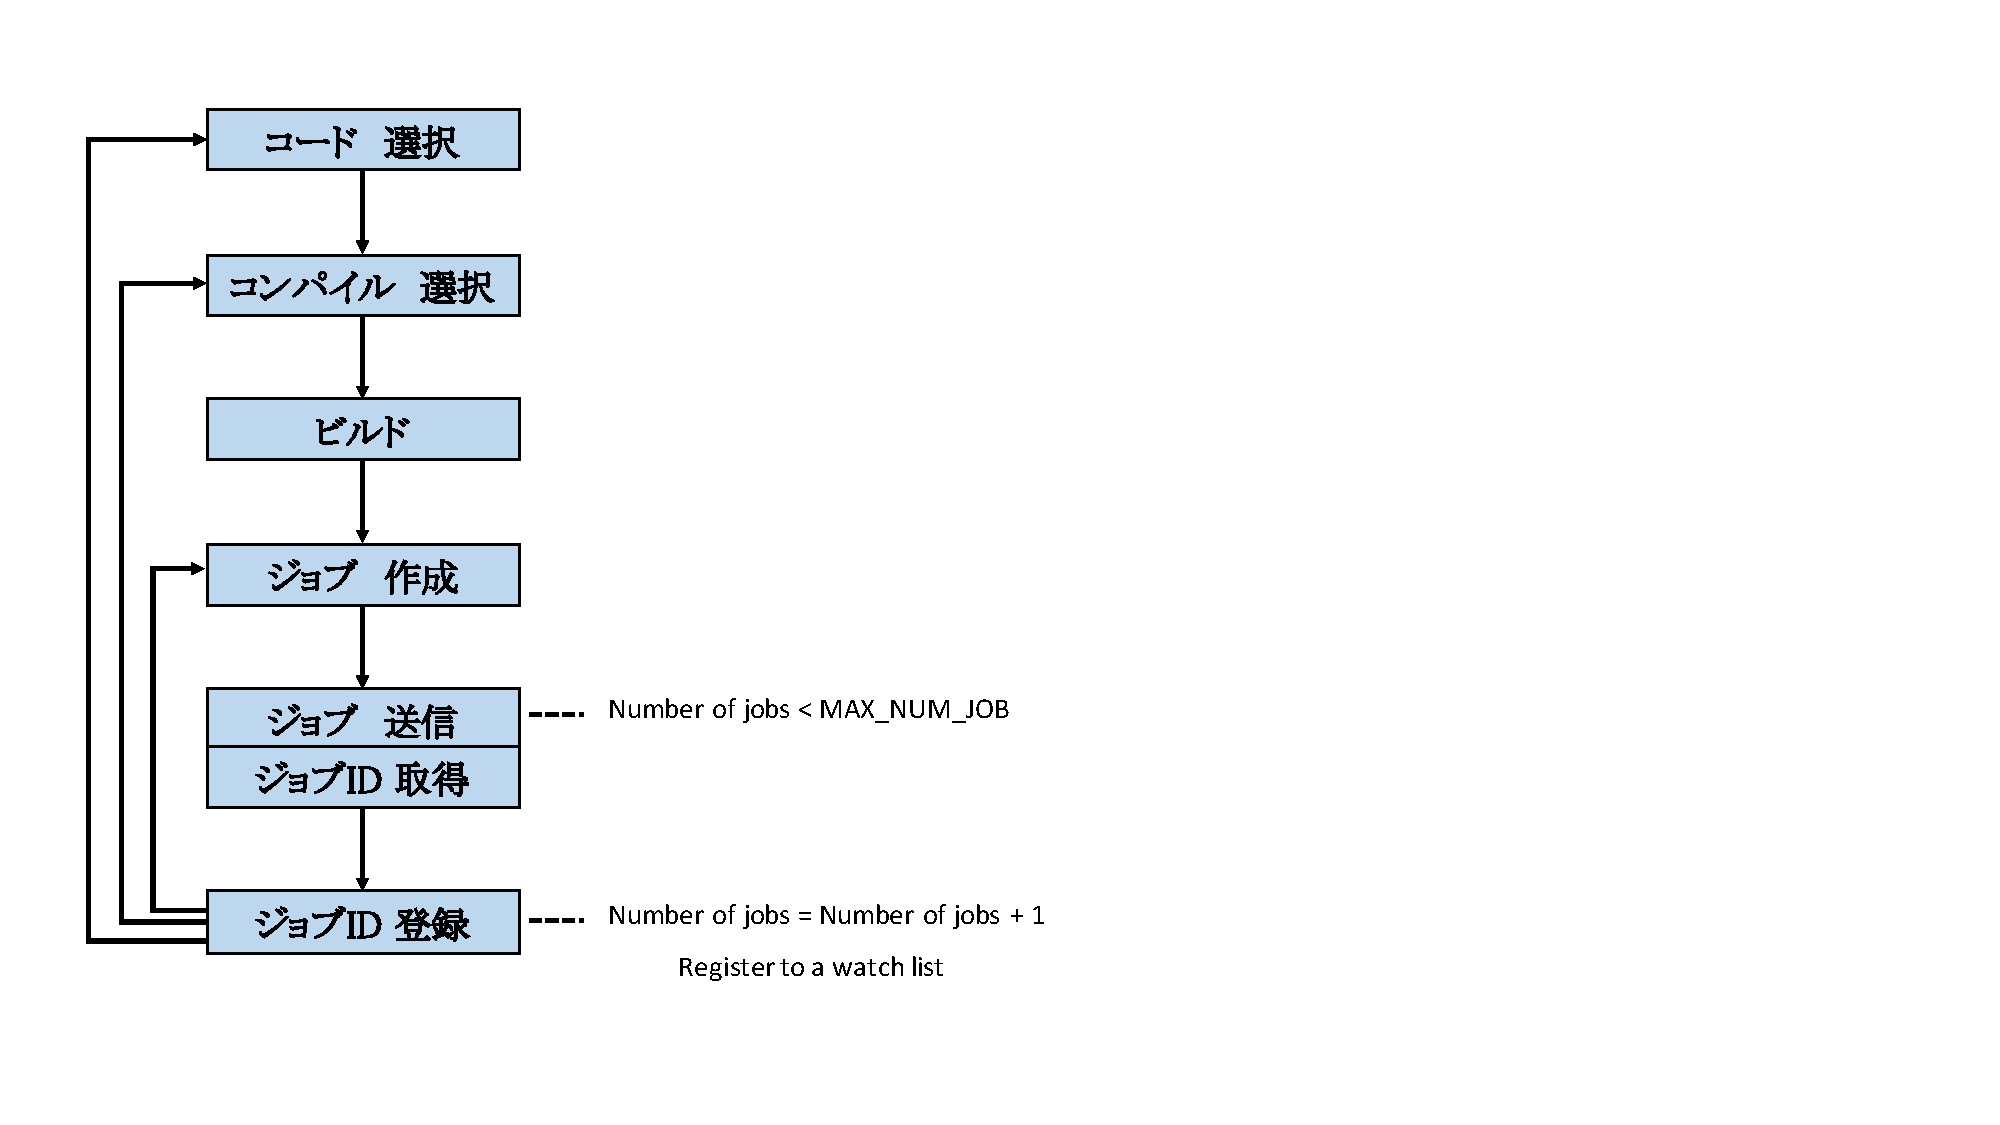
\includegraphics[width=20.0cm]{./images/state.pdf}
    \caption{シミュレータ 状態遷移図}
    \label{fig:test}
  \end{center}
\end{figure}
{\footnotesize
\lstinputlisting[caption=シミュレータ疑似コード,label=hogehoge,frame=single]{src/pseudocode/simulator}
}
疑似コードで示した通り,シミュレータは逐次パラメータを選択し実行形式とジョブスクリプトを多数のパラメータ候補群の中から生成するループ,
ジョブの同時実行数を制限しつつ,作成したジョブをジョブキューに登録する実行,
そして実行中のジョブを監視し,完了した段階でその結果を集約し使用したパラメータとともに保存する記録の3つの機能から成立している.\\
以下にそれぞれの機能について詳細を示す.\\
\paragraph{全体ループ}~\\
疑似コード内の8-22行目までが全体のループを構成している.\\
{\footnotesize
\lstinputlisting[caption=シミュレータ 全体ループ,label=hogehoge,frame=single, firstline=8, lastline=22]{src/pseudocode/simulator}
}
ループ内部では,プログラムのビルド,ジョブスクリプトの生成,そして生成した実行形式とジョブスクリプトをジョブキューにdeployするという3つのことを行っている.\\
プログラムのビルド,ジョブの実行に比べジョブスクリプトの生成にかかる時間は無視できる程度のものであるため,ジョブスクリプトの生成をもっとも内側のループに持ってきた.\\
これにより,ジョブキューでジョブが実行されるのを待っているうちにビルドを行うことができ,全体としてシミュレーションの時間を減らすことが期待できる.\\
\paragraph{ジョブ実行}~\\
{\footnotesize
\lstinputlisting[caption=シミュレータ ジョブ実行,label=hogehoge,frame=single, firstline=24, lastline=29]{src/pseudocode/simulator}
}
スーパーコンピュータ京のような複数のユーザーが用いるシステムにおいて,ジョブを一度に大量に投げるのは好ましくない.\\
そのため,ジョブをジョブキューに投げる前に事前に設定した最大同時ジョブ実行数と現在の実行中のジョブの数を比較し,最大数と同数なのであれば待機する処理が必要である.\\
本研究では,グローバル変数として現在実行中のジョブのIDを保持するリストを定義し,そのリストの数と比較することで実現している.\\
また,後述するジョブ結果の集約においてこのジョブIDを保持するリストは別スレッドから参照されており,リスト内のジョブが完了した段階でmutexによってロックされた上で更新される.\\
\paragraph{ジョブ結果の集約}~\\
{\footnotesize
\lstinputlisting[caption=シミュレータ ジョブ結果の集約,label=hogehoge,frame=single, firstline=31, lastline=37]{src/pseudocode/simulator}
}
様々なパラメータの組の中から最適な組み合わせを選びたいため,それぞれのジョブの結果とパラメータの組を結びつける必要がある.\\
ジョブが完了したか否かは,ジョブの状況を取得するコマンドを利用することで得ることができる.\\
次にスーパーコンピュータ京と研究室クラスタで上記のコマンドを実行した結果を示す.\\
{\footnotesize
\begin{lstlisting}[numbers=none]
京
>> pjstat
a


研究室クラスタ
>> qstat
Job ID  Name  User  Time  Use S Queue
--- --  ----  ----  ----  --- - -----
3381.cluster  job_cluster.sh  inoue 00:44:33  C cluster
3383.cluster  job_cluster.sh  inoue 00:23:59  C cluster
3384.cluster  job_cluster.sh  inoue 00:47:37  C cluster
3385.cluster  job_cluster.sh  inoue 00:24:02  C cluster
3386.cluster  job_cluster.sh  inoue 00:23:57  C cluster
3387.cluster  job_cluster.sh   inoue           00:47:32 C cluster
3388.cluster               job_cluster.sh   inoue           00:24:07 C cluster
3389.cluster               job_cluster.sh   inoue           00:24:01 C cluster
3390.cluster               job_cluster.sh   inoue           00:18:33 R cluster
3391.cluster               job_cluster.sh   inoue 0 R cluster
3392.cluster               job_cluster.sh   inoue                  0 Q cluster
3393.cluster               job_cluster.sh   inoue                  0 Q cluster




\end{lstlisting}
}
\subsubsection{モデルに依存するパラメータ}
